%   MSc Business Analytics Dissertation
%
%   Title:     Literature Review
%   Author: Conor Reid
%
%   Chapter 3: Literature Review
%
\chapter{Literature Review}\label{C.LitReview}
\section{Introduction}\label{S.intro3}
{It is natural in business to seek to optimise all aspects of corporate activity, with a view to positively effecting economic outcomes. This is reflected in the literature on this domain, which considers the problem in a number of different forms, following a wide range of methodologies and reaching quite different results at times. A review of a snapshot of this literature included here. \\\\
First, some of the ways that corporate success can be quantified is presented. This includes how success is defined by \cite{moldovan2015learning}, as well as by others whose approaches may benefit this study. Also included here is a discussion of various fronts on which companies act, such as their corporate social responsibility commitments, with a view to including these aspects in this analysis as independent explanatory features. This is followed by an analysis of existing literature on the relationship between corporate governance and company performance, again including the work of \cite{moldovan2015learning} as well as other relevant studies. Then, an exploration is carried out of the literature regarding causation and the statistical techniques used to infer causation, with consideration of how these can be realised in this domain. There is also discussion on the issues that arise in attempting to do so, and how they can be addressed. This chapter finishes with a summary of the research gap that this study aims to address. }
\section{Company Performance - Measures and Influencers}\label{comPerform}
\subsection{Introduction}
{Among the key aspects of this study is the quantifying of corporate success, in a way that accurately represents {\it "good"} and {\it "bad"} corporate performance. There are many ways to do this, one of the most simple of which is to use financial ratios. Uncountable ratios have developed, each attempting to assign numerical performance ratings to companies and differing from one another by the accounting indictors considered and the aggregation of these indicators. \cite {eidleman1995z} outlines the patterns that ratios tend to follow. He states that these ratios are mostly created by academic researchers, who constantly derive new ways of combining individual metrics together to facilitate meaningful comparison between companies. First, researchers find a sample of companies that meet some predetermined criterion of failure, as well as another sample of comparable firms (size, industry etc) that differ only in financial health. A number of ratios are developed and tested against this dataset to determine which returns values that are consistently and significantly different for each group. Those which do so successfully are kept, the rest are discarded. Weights are assigned to each ratio to reach an aggregate equation. New firms are scored, and real-world performance recorded to measure how useful the new ratios are in practice. \\\\
This study primarily considers corporate governance features as predictors of corporate economic success. This follows the lead of \cite{moldovan2015learning} who do the same. Having said this, an aim of this study is to expand the range of predictors considered, and to this end we discuss alternative sources of company data that can be incorporated into the model. Perhaps the inclusion of more varied and diverse independent features, such as a companies social responsibility commitments or their impact on the environment can enhance overall understanding in this domain. These areas are discussed in this chapter.    }
\subsection{Financial Ratios}\label{FinancialRatios}
{Some financial ratios are more useful than others, varying significantly in complexity, in what particular aspects of a company they consider and also in how they combine those measures. This section includes a discussion of some of the most commonly used ratios, with comments on how best they can be used and in what context they are most powerful. \\\\
One of the indicators of corporate economic performance used by \cite{moldovan2015learning} is Tobin's Q score. This measure was devised by \cite{tobin1969general} who postulated that the combined market value of a given company should be equal to their replacement costs. When a companies replacement cost is equal to its market value, it is said to be in an ideal state. Any deviation either way, a ratio above or below 1, indicates future investment or the selling of assets respectively. \cite{moldovan2015learning} argue that the Q score allows the estimation of intangible assets, and is thus a worthy inclusion as a dependant measure of corporate success. Intangible assets drive market value up, rising the Q score.  \\\\
The use of this measure is well established in the literature, by \cite{chung1994simple}, 
\cite{bhagat2008corporate} and \cite{bolton2011unified}. \cite{chung1994simple} state that Tobin's Q plays an important part in financial interactions, and is employed to explain diverse corporate phenomena during the  decision making process for investment opportunities. \cite{bolton2011unified} used Tobin's Q to propose a model for dynamic investment and risk management and found that investment is best driven by an aggreagte model of which the Q score plays an important role. \\\\
The formal definition of Tobin's Q is presented by \cite{chung1994simple}, along side a much more simplified and conservative approximation of the authors making. This less complex definition is seen commonly in literature, for example by \cite{wahba2008does}. This formulation is given below as; \\
\begin {equation}\label{TobinQ}
(Approximate) \quad q  = \small {\frac{MVE + PS + DEBT}{TA}}
\end{equation}\\
Here, $MVE$ represents the product of a companies share price and count of common outstanding stock shares. $PS$ represents the liquidating value of the companies preferred stock. $DEBT$ represents the companies short-term liabilities minus its assets, also short-term. Finally, $TA$ represents the book value of the total assets of the company. In layman terms, assets that cannot be easily quantified can not always be entered in a companies books, but do always contribute to the share price of that company. Thus, a firm with lots of this type of asset will have a high Q score, and those without will have a low score.\\\\ 
There is debate as to the practically of the Q score. Intuitively, the Q score places a very high importance on one specific aspect of a business. For example, before WhatApp was acquired by Facebook it had very little concrete physical assets (i.e. those that could be recorded in their accounts). Rather, it had a platform with approximately 400million users, and a very high Q score. After purchase, the Q score would have dropped significantly since the amount Facebook paid would become the concrete asset recorded in their books. This is not to say that the Q score is a bad success indicator, but rather it may not fully represent the real value of a company at a given time.\\\\    \cite{chung1994simple} state in their research that the Q score is often neglected in real-world situations. One of the reasons they give for this is the complexity of the necessary calculations, and a potential unfamiliarity with its operational intricacies. Another reason is the unavailability of relevant data, particularly of sufficiently high accuracy and instantaneous availability. To counteract this, they worked to create and test an accurate approximation of Tobin's Q that utilises only basic financial information, show in equation \ref{TobinQ}.  They conclude that their approximation is close enough to the more formal definition to be used where more exhaustive calculations are not possible. \\\\
%\cite {dybvig2010tobin} criticise Tobin's Q more strongly, stating that it is fundamentally malformed as a measure of corporate performance. They highlight long-serving managers as risk adverse, and who "...can {\it enjoy the quiet life} and underinvest". A logical implication of this is that firms invest less and operate well below their profit-generating capacity and thus reduces their net-present value. However, such is Tobin's Q formulated, underinvestment by a firm increases its Q score. They go on to explain the scores ambiguity, COME BACK TO. \\\\
Another measure of corporate success used by \cite{moldovan2015learning} is the Altman Z score, which can be used as a probabilistic measure of whether a company will fall into bankruptcy within the next two years. It can also be used more generally as a financial distress measure and to predict corporate defaults. The authors point out that there is much advocacy in the literature for using this measure, and this study was unable to find any that strongly reject its usefulness. The Altman Z score is given as;
\begin {equation}\label{AltmanZScore}
\begin{aligned}
Z \ Score \quad = \quad & 1.2\bigg(\frac{Working \ Capital}{Total \ Assets}\bigg) \ + \\\\
		& 1.4\bigg({\frac{Retained \ Earnings}{Total \ Assets}}\bigg) \ + \\\\
		& 3.3\bigg({\frac{Earnings \ before \ Interest \ and \ Tax}{Total \ Assets}}\bigg) \ + \\\\
		& 0.6\bigg({\frac{Market \ Value \ of \ Equity}{Total \ Liabilities}}\bigg) \ + \\\\
		& 1.0\bigg({\frac{Sales}{Total \ Assets}}\bigg)
\end{aligned}
\end{equation}\\
Among those that support this scores use is \cite {eidleman1995z}, who discusses its use in practice. He begins by highlighting Altman's own tests using the Z score which involved predicting 72\% of bankruptcies two years prior to the event, although the sample size or companies involved are not mentioned. Eidleman argues that the Z score is tried and tested, and ``it has been demonstrated to be quite reliable in a variety of contexts and countries.'' \cite {eidleman1995z}. \\\\
Eidleman also outlines circumstances that warrant corrections and alterations to equation \ref{AltmanZScore}, in order to generalise it beyond its originally intended means. He argues that before being able to use the Z score, one must ensure the company in question is comparable to those involved in Altman's original study. Altman considered manufacturing and small firms in his original analysis, thus corrections must be made before scoring companies in different industries. Eidelman points to two specific circumstances here. \\\\
The first considers privately held companies, whose stocks are no publicly traded meaning term four of equation \ref{AltmanZScore} cannot be calculated. To correct for this, the Z score can be re-estimated using book values of equity. In other words, details from balance sheets published by private firms voluntarily can be used rather than details gleamed from the stock market. Certainly a work-around here is to consider solely publicly traded companies. A consequence of this is that such an analysis would only include companies that are bound by the the corporate governance code in their jurisdiction, which would need to be taken into account in studies such as this one.\\\\ Eidleman's second consideration is for non-manufacturing firms. The fifth term of equation \ref{AltmanZScore}, according to Eidleman, varies significantly by industry. He argues that merchandise firms for example, are significantly less capital intense and thus are much more likely to enjoy higher asset turnover and consequently Z-Scores. Z scores then would be likely to under-predict bankruptcy in these cases. In order to correct for this, a recommendation comes from Altman to eliminate the fifth term and adjust the weights. 
\clearpage
The adjusted equation \ref{AltmanZScoreAjusted} is shown below;
\begin {equation}\label{AltmanZScoreAjusted}
\begin{aligned}
Z \ Score \quad =  \quad & 6.56\bigg(\frac{Working \ Capital}{Total \ Assets}\bigg) \ + \\\\
		& 3.26\bigg({\frac{Retained \ Earnings}{Total \ Assets}}\bigg) \ + \\\\
		& 6.72\bigg({\frac{Earnings \ before \ Interest \ and \ Tax}{Total \ Assets}}\bigg) \ + \\\\
		& 1.05\bigg({\frac{Market \ Value \ of \ Equity}{Total \ Liabilities}}\bigg) \ \\\\ 
\end{aligned}
\end{equation}\\
Overall, the Altman Z score seems a highly appropriate indicator of corporate financial strength and thus success, and one that should be considered in this study. Consideration will need to be had for the type of industry included in this analysis, that will inform the exact calculation of the Z score itself. }\\\\
{As mentioned above, both Tobin's Q score and the Altman Z score were used by \cite{moldovan2015learning}, and are to be included in the current studies to emulate their work. However, one of the goals of this study is to extend this work by including other measures of corporate success or health. An exploration of the Beneish M-Score is carried out with this in mind. The Beneish M-Score is an aggregate financial ratio calculated using standard accounting data and acts as a probabilistic measure of intentional manipulation of a companies declared earnings. This score has been used in many studies aiming to detect corporate fraud and deception, or more generally and in combination with other factors to detect financial distress before it happens. \cite{beneishCost} state that although the risk of significant financial loss as a result of financial reporting fraud is huge, investors spend little time utilising publicly available data in an effort to detect that fraud. Thus, this ratio is a worthy addition to this study. }\\\\
{\cite{beneishOG} calculates the M-Score using the following formula \ref{MScore}.
\begin {equation}\label{MScore}
\begin{aligned}
M \ Score \quad =  \quad & -4.84 + 0.920(DSRI) + 0.528(GMI) \ + \\\\ 
		& 0.404(AQI)+ 0.892(SGI) + 0.115(DEPI) \ - \\\\
		& 0.172(SGAI) + 4.679(TATA) - 0.327(LEVI)  \ \\\\
\end{aligned}
\end{equation}\\
where
\begin {equation}\label{MScore-DSRI}
\begin{aligned}
DSRI = \bigg( \frac{Receivables_t}{Sales_t} \bigg) / \bigg( \frac{Receivables_{t-1}}{Sales_{t-1}} \bigg) 
\end{aligned}
\end{equation}\\
The days sales in receivables index (DSRI) measures the amount of days that sales are in accounts receivable in a year compared to the previous year. A ratio of much greater than 1 coupled with a slower growth in sales could be an indication of inflated revenues. 

\begin{equation}\label{MScore-GMI}
\begin{aligned}
GMI = \bigg( \frac{Sales_{t-1} - Costs of Goods Sold_{t-1}}{Sales_{t-1}} \bigg) / \bigg( \frac{Sales_{t} - Costs of Goods Sold_{t}}{Sales_{t}} \bigg)
\end{aligned}
\end{equation}\\
The gross margin index (GMI) measures the ratio of current and previous years gross margin, with an index much greater than 1 signalling that gross margin has declined in the period, which according to \cite{mahamaCorpFraud} could provide motivation for manipulation. Lower gross margins are linked to lower future earning, which \cite{beneishCost} state is linked to higher probabilities of manipulation.     

\begin{equation}\label{MScore-AQI}
\begin{aligned}
AQI = \bigg( 1 - \frac{Current Assets_t + PPE_t}{Total Assets_t} \bigg) /  \bigg( 1 - \frac{Current Assets_{t-1} + PPE_{t-1}}{Total Assets_{t-1}} \bigg)
\end{aligned}
\end{equation}\\
The asset quality index (AQI) measures asset quality as a ratio of non-current assets (less property plant and equipment) to total assets from one year to the next. A ratio higher than 1 indicates that the company may be involved in cost deferral. A deferred cost is one that in incurred but not charged to expense until a later reporting period, and thus could be a sign a risky behaviour.   

\begin{equation}\label{MScore-SGI}
\begin{aligned}
SGI = \bigg(\frac{Sales_t}{Sales_{t-1}} \bigg) 
\end{aligned}
\end{equation}\\
The sales growth index (SGI) is a simple ratio of sales from year to year. \cite{beneishOG} states that while growth is not inherently a sign of manipulation, growing firms are viewed as more likely to commit financial reporting fraud due to the pressure placed on managers to reach earnings targets. The authors go on to argue that small, high growth companies stand to lose more in the face of slowing growth figures than their more mature counterparts, leading to potentially risky behaviour.  

\begin{equation}\label{MScore-DEPI}
\begin{aligned}
DEPI = \bigg(\frac{Depreciation_{t-1}}{Depreciation_{t-1} + PPE_{t-1}} \bigg) /   \bigg(\frac{Depreciation_{t}}{Depreciation_{t} + PPE_{t}} \bigg)
\end{aligned}
\end{equation}\\
The deprecation index (DEPI) is a ratio of the rate of deprecation from year to year. A ratio greater than 1 signals that the rate at which assets are losing value has decreased, potentially as a result of management revising upwards their estimates of viable serviceable lifespan. \cite{beneishOG} states that there should be a positive correlation between this ratio and the likelihood of a company manipulating earnings reports.     

\begin{equation}\label{MScore-SGAI}
\begin{aligned}
SGAI = \bigg(\frac{SGA Expenses_{t}}{Sales_{t}} \bigg) /  \bigg(\frac{SGA Expenses_{t-1}}{Sales_{t-1}} \bigg)
\end{aligned}
\end{equation}\\
The sales general and administrative expenses index (SGAI) is calculated as the ratio of general sales and administrative expenses to sales from year to year. \cite{beneishOG} expect a positive corrolation between this score and likelihood to commit reporting fraud.  

\begin{equation}\label{MScore-TATA}
\begin{aligned}
TATA = \bigg(\frac{\Delta Working Capital_t - \Delta Cash - \Delta Income Tax Payable - Depreciation }{Total Assets} \bigg) 
\end{aligned}
\end{equation}\\
Total accruals to total assets (TATA) is a proxy ratio for the extend to which cash underlies reported earnings. Total accruals are calculated as the change in working capital accounts (other than cash) minus depreciation. Higher accruals are thus an indication of less cash, and should be associated with a higher risk of reporting fraud.  

\begin{equation}\label{MScore-LEVI}
\begin{aligned}
LEVI = \bigg(\frac{LTD_t + Current Liabilities_t }{Total Assets_t} \bigg) /  \bigg(\frac{LTD_{t-1} + Current Liabilities_{t-1} }{Total Assets_{t-1}} \bigg)
\end{aligned}
\end{equation}\\
Finally, the leverage index (LEVI) is a ratio of total debt to total assets from year to year, with a value greater than 1 an indicator of an increase in leverage over the period. \cite{beneishOG} state that this is associated with the probability the company will default, or in other words be unable to make the required payments on their debt obligations. }\\\\
{\cite{mahamaCorpFraud} uses the Beneish model, interestingly in conjunction with the (five variable) Altman Z model seen above, to show that the Enron scandal could have been detected as early as 1997, well before the company filed for bankruptcy in 2001. This was done using data from the United States State Examinations Commission (SEC) spanning from 1996 to 2000. As has been mentioned above, an Altman Z score below 1.81 indicates company is at high risk of bankruptcy. Here, an M-Score greater than -2.22 is an indication of manipulated financial reporting. Applying this logic to Enron, the author compiled the below table
\begin{table}[h!]
\centering
\begin{tabular}{ |p{2cm}||p{1.2cm}|p{1.2cm}|p{1.2cm}|p{1.2cm}|p{1.2cm}|p{1.2cm}|  }
 \hline
 Metric & 2001 & 2000 & 1999 & 1998 & 1997 & 1996\\
 \hline
 Z-Score &  & 2.481  & 3.040 & 2.029 & 1.611 & 1.884  \\
 M-Score & -2.358  & -0.343 & -1.323 & -2.426 & -2.064 &  \\
 \hline
\end{tabular}
\caption{Enron Scandal - \cite{mahamaCorpFraud}}
\end{table}\\\\
Immediately obvious here is that Enron was in a state of bankruptcy in 1997, while in subsequent years it hovered above that threshold in a grey area of bankruptcy risk. The M-Score shows us that Enron was likely commiting fraud from 1998, a year after experiencing their worst Altman Z score. \cite{mahamaCorpFraud} state that being brought so close the bankruptcy in 1997 lead to manipulation of financial reporting a year later.}\\\\
{\cite{herawatiBeneish} studies the utility of the Beneish M-Score in detecting financial fraud, specifically using data released by the Financial Services Authority in the United Kingdom relating to companies that are known to have committed fraud during the period of 2011-2014. This amounted to 35 companies, with a further 35 added to the study and picked based on equality of assets and type of industry. The author constructed a logit regression model, using a binary indicator as the dependent variable that represented the presence of fraud or not. The aim then was to find the weightings of each sub-ratio within the M-Score to first analyse its aggregate ability to detect fraud but also the utility of each of the subcomponents. The results of this analysis are shown in figure \ref{beneish_comp}. 
\begin{figure}[h] \label{logitBeneish}
\centering
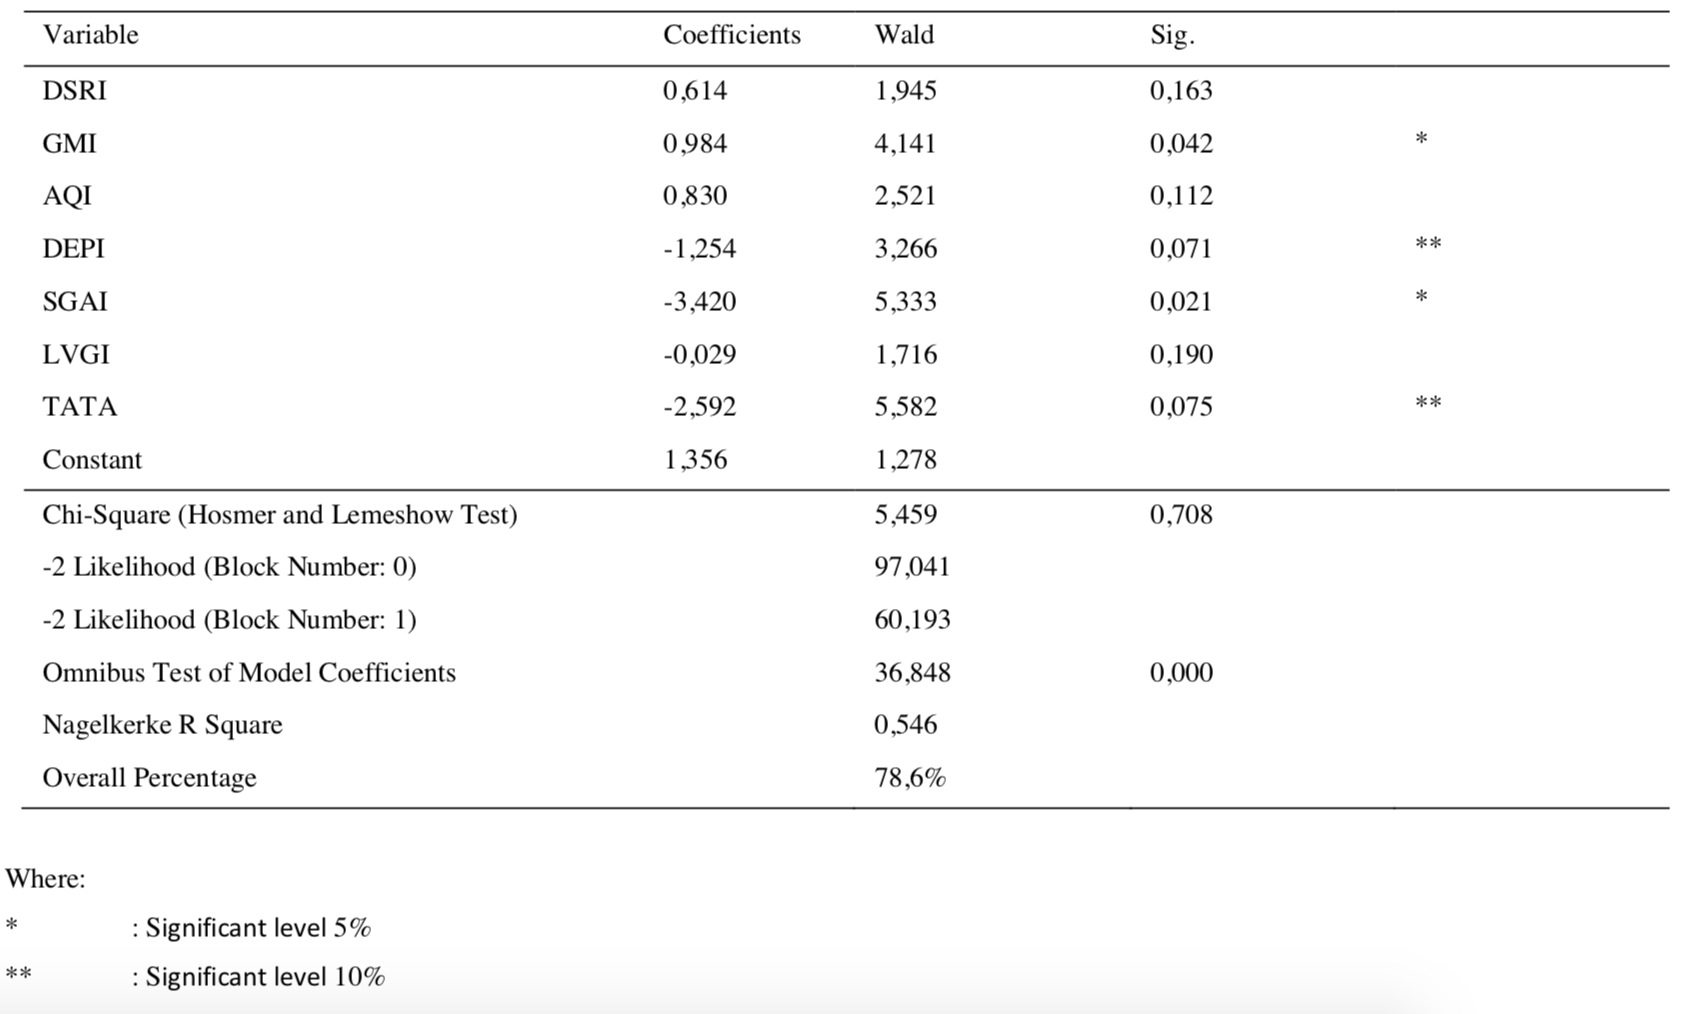
\includegraphics[scale = 0.7, angle =90]{images/litReview/beneish_comp.png}
\caption{Logit Regression for Beneish M-Score (Source: \cite{herawatiBeneish}).}
\label{beneish_comp}
\end{figure}\\\\
It's clear form this table that the sub-ratio's GMI, DEPI, SGAI and TATA are all statistically significant and have non-negligible weights. All of DSRI, AQI and LVGI do not and so are less likely to be influential in detecting the presence of financial reporting fraud. Its clear from this study that the Beneish M-Score is a useful metric for analysing the activity of a company and measuring performance on a different dimension than considered here previously.  }\\\\
\clearpage
{\cite{kamalDetection} also use the Beneish M-Score to detect earnings manipulation and financial statement fraud in a group of Malaysian public list companies, thus extending its use beyond the context of the United States. Here, the authors gathered data on 17 companies that were, between 1996 and 2014, prosecuted by the Securities Commission Malaysia for commuting such acts of misreporting and intensional obfuscation. They calculated the M-Score for each company in the years prior to each prosecution, and found that in 14 cases (or 82\%) the scores were less than the threshold and would have raised alarm at the time. Figure \ref{kamalBeneish} shows the numerical findings of \cite{kamalDetection}. 
\begin{figure}[h] 
\centering
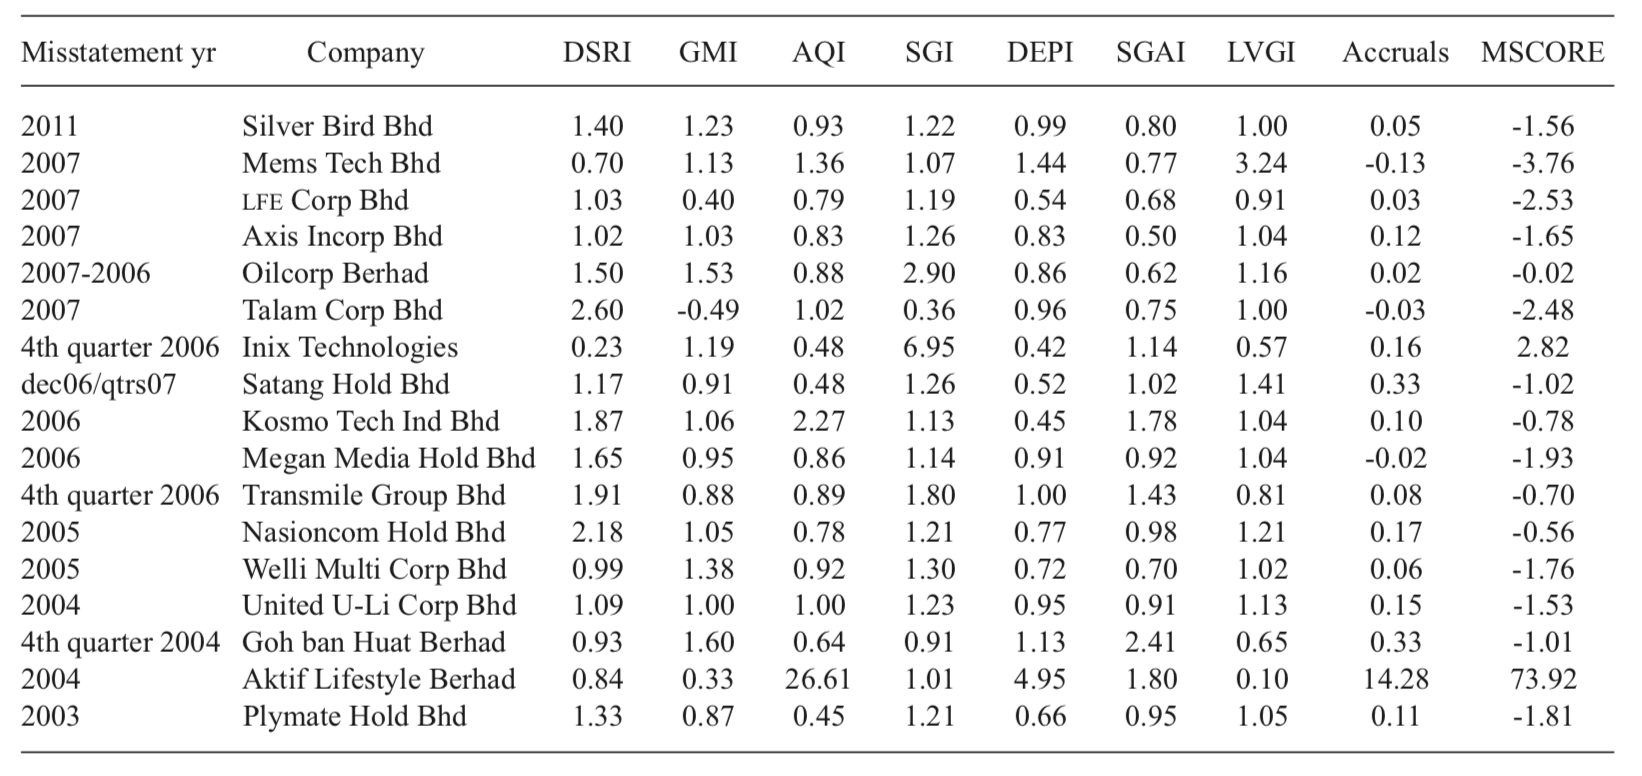
\includegraphics[scale = 0.7, angle =90]{images/litReview/kamalBeneish.png}
\caption{Beneish M-Score for Prosecuted Malaysian Companies (Source: \cite{kamalDetection}).}
\label{kamalBeneish}
\end{figure}\\\\
While the authors here present strong evidence as to the utility of the M-Score in detecting malpractice, it is just as interesting to look at the companies that presented so-called "safe" scores but in actuality proved to be fraudulent. As mentioned previously, a score of less than -2.22 (a greater negative) would classify a company as "safe". There are three such companies here, with the lowest M-Score of -3.76 for a company called Mems Tech Bhd. Interestingly, the LVGI score here is noticeably higher than for all other companies, with the net effect of this component acting to drive the overall M-Score down (since it's multiplier is negative) and reducing the calculated risk. Since we know this company was in fact convicted of fraud, this evidence supports the findings of \cite{herawatiBeneish} that the LVGI score may not be so useful in overall fraud detection. }
\clearpage
\subsection{Environmental Considerations}\label{EnvironmentalConsiderations}
{As mentioned previously, there is likely much room for improvement in the range of predictors of success considered in this analysis. One potentially useful area to consider is the environmental performance of the company, studied by \cite{schaltegger2002link}. The authors primary focus is on environmental management, specifically as a vehicle for corporate success. It is assumed here that environmental management and performance relate to the controlling of costs relating perhaps to the mining of natural resources. This may also refer to fines, penalties or taxes that are incurred due to harmful emissions, which must be carefully managed within a company to mitigate against. \\\\
The authors present two conflicting viewpoints in this space. The first states that improved environmental performance predominantly causes an increase in operating costs, due to investment and so on which in turn negatively effects the profitability of the company. The second viewpoint states the opposite; improving a firms environmental performance in fact induces cost savings, which drives increases in profitability. Interestingly, the authors present opinions that environmental investment often both negatively increases costs and positively increases income. Having said this, they argue that such a direct link is not present in practice, and that instead it is the identification and management of the relationship that is more important. The conflicting viewpoints are visualised in figure \ref{ch3_successAndEnviornment}. 
\begin{figure}[h] 
\centering
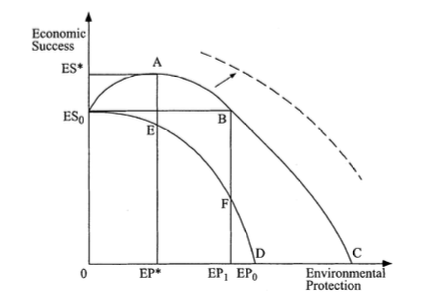
\includegraphics[scale = 0.7]{images/ch3_successAndEnviornment.png}
\caption{Correlation between corporate environmental protection spending and economic success (Source: \cite{schaltegger2002link}).}
\label{ch3_successAndEnviornment}
\end{figure}\\\\
$ES_0$ on the vertical axis represents the current level of economic success, described by the authors a certain shareholder value. According the the pessimistic view of environmental spending, this value decreases as spending in environmental protection increases (through points E and F, to D where non profit can be made). That is, spending in this space reduces profit making ability to eventual zero. The more optimistic view is represented by the path from $ES_0$ through points A and B to point C (again where no profit is possible). This represents the ideology that some economic gain can be achieved, at least to some degree before tailing off, by being environmentally conscious. Of course, even in this situation there is an optimal investment level, after which profit making ability decreases. \\\\
The authors draw point to two important ideas, derived from figure \ref{ch3_successAndEnviornment}. First, they argue that environmental performance can vary at a given level of economic success. It is both possible to be equally successful by being either environmental friendly or harmful. This indicates that investment in this space does not necessarily mean poor economic performance. Secondly, the reverse; that economic success can vary for a given level of environmental protection. That is, being environmentally conscious is no guarantee of economic benefit. The authors reiterate that the correlation between economic and environmental performance depends on not just company externalities but internal variables which are influenced by management. It is firm management, who moderate this relationship, that must be optimised in order to gain economically. The authors put this forward as an group of explanatory covariates not considered in the literature to this point. \\\\
It is natural then to ask how environmental management can be quantified in data for analysis. \cite{schaltegger2002link} suggest two cases for deriving data. The first relates to the firms ability to utilise to the full the economic benefits of environmental protection measures. This may materialise in R\&D spending, or other marketing positioning that communicates their efforts and establishes the company as industry leaders. They are seen as quality leaders, with their environmental management policies a significant driver of this. The second case relates to how this reputation is achieved in practice, by realising the optimal environmental performance for maximum economic success. This can take the form of identifying and implementing optimise production processes for example, facilitated by the identification of opportunities and "eco-efficiency potentials". \\\\
\cite{wahba2008does} also performs research in this area, studying whether the market values corporate environmental responsibility, specifically in an Egyptian context. Similarly to \cite{schaltegger2002link}, the author acknowledges divided and inconclusive literature on this topic, stating an aim to present empirical evidence on how engagement with environmental responsibility can positively influence corporate market value. This analysis looks at a sample of 156 firms across 19 industries, using the market value of a firm as the dependant variable (interestingly, quantified by Tobin's Q score mentioned previously). Important to note is the authors use of ISO 14000/14001 certification as a proxy for environmental performance. This is recognised by the authors as non-ideal, however this may still have some utility in future research to address the difficulty in quantifying performance in this area. \\\\
An interesting and important consideration is made by \cite{wahba2008does}. She states that companies with greater economic success have a greater ability to invest in environmental endeavours, leading to a theory that the two may be jointly determined. This theory is tested before regression analysis run. To do this, the author uses the specification test of \cite{hausman1978specification} to test for endogeneity. Endogeneity occurs in econometrics when an explanatory variable correlates with the error term, rather than some other feature. \cite{wahba2008does} states that the result of this analysis is that endogeneity is not occurring, but points to an important consideration that the current study may need to take into account. One of the common causes of this is a causal loop between an independent and a dependant variable, and can obviously lead to wildly inaccurate results. \\\\
 \cite{wahba2008does} state that the overall finding of this research is that the market does in fact reward firms for their environmental efforts, by positively influencing that firms Tobin's Q score, but do point to similar issues raised by \cite{schaltegger2002link}. Namely, that a companies decision to reduce their impact on the environment comes with significant cost and that if this is not managed correctly, the economic benefits evaporate.     \\\\
There is clear support in the literature for the presence of a relationship between corporate economic success and environmental performance. \cite{schaltegger2002link} suggest it is the firm management of environmental considerations that influences success, and put this forward as an explanatory variable not yet considered in literature. This theory is supported by \cite{wahba2008does}, who find a strong relationship in this space but with a caveat that management plays a significant role in realising benefits. It remains to be seen exactly how this can be realised in data analysis, and what family of covariates could be incorporated into the model.}
\subsection{Corporate Social Responsibility} \label{CorporateSocialResponsibility}
{Corporate social responsibility, or CSR, is defined by the European Commission as "the responsibility of enterprises for their impacts on society". This is similar to being conscious of environmental impact, but is more generalised to include compliance with established ethical standards and national and international norms. Central to CSR is the creation of shared value between themselves, their stakeholders and larger society as well as mitigating possible adverse events with those groups. It is natural to consider elements of CSR then, when discussing predictors of firm success. \\\\
\cite{orlitzky2003corporate} perform meta-analysis in the link between corporate social and financial performance. They begin by stating;
``Most theorising on the relationship between corporate social / environmental performance (CSP) and corporate financial performance (CFP) assumes that the current evidence is too fractured or too variable to draw any generalisable conclusions \cite{orlitzky2003corporate}.''\\\\
Their research aims to show this claim is unfounded, and that it is indeed possible to derive insight in this space by providing a more rigorous methodology for drawing such conclusions. They argue that researchers have attempted to find causal relationships between CSP and CSR, but have failed in part due to a failure to see vital differences between theory and operational applications. They also state that an aim of their research is to aggregate knowledge in the area, and highlight important findings they believe to be overlooked. This type of meta-analysis have been proven to provide value by considering a number of disparate and conflicting results holistically, by reaching an aggregate conclusion.\\\\
They present a number of hypotheses about the influence of CSP. They first state that CSP and CFP are positively related, regardless of industry and the context of the given study relating the two. They base this on a number of studies, stating that CSP is a vital form of "good management theory" that boasts competitive advantage by addressing stakeholder concerns quickly and fairly.  Secondly, they hypothesise on the temporal nature of this relationship, and further that there is a bidirectional causality between CSR and CFP. That is, there is a circular and virtuous causal relationship that governs performance in each area. This is supported by the idea that prior success in CFP facilitates positive engagement in CSP, due to increased responsibility and freedom at the managerial level. This conclusion mirrors that seen in section \ref{EnvironmentalConsiderations}, where it was theorised that increased economic success drives better environmental performance.\\\\
The third hypothesis put forward by \cite{orlitzky2003corporate} involves the underlying logic behind the correlation between CSP and CFP. The first is that CSP boasts managerial competencies and organisational efficiency, by enabling shared knowledge of the firm's market as well as social and political environments. Secondly they suggest that CSP is a driving factor behind the firm's reputation, and thus elicits significant goodwill from stakeholders. \\\\
The fourth and final hypothesis put forward involves the methodology used by previous studies to draw conclusions from. The authors here suggest that the variance in results seen across studies can be explained by sampling or measurement error, for example. \\\\
In order to support these claims, \cite{orlitzky2003corporate} perform a meta-analysis involving 52 studies across both CSP and CFP, resulting in a total sample size of 33,878 observations on which they perform their analysis. This analysis involves a statistical aggregation technique to be applied, which calculates the cumulative correlations across studies, correcting for variable elements of those studies to reach one "true score correlation ($\rho$)". Using this technique, the authors were able to explain 24\% of the cross-study variance in relation to the observed r value, which they suggest is significant. That is, by controlling for sampling and measurement errors across multiple studies, they could reduce the variation in results by 25\%. They suggest that this, strengthened with other analysis, supports their collection of hypotheses.\\\\
The authors compare their results with others who performed similar research. Key to this comparison is a discussion regarding the linkage between CSP and CFP. That state that other researchers have traditionally been concerned with the "Halo effect". That is, that correlation found (that CSP influences CFP) are due to the experimental procedure or are spuriously perceived. The authors here dismiss this, stating that the only logical halo link would be in the reverse direction. That is, that a company who are high financially successful may be scored highly in CSP regardless of factual information in that regard. They go further, and state that even this hypothetical (but more logical) argument is debunked by their meta-analysis which shows a strong directional (or temporal) link between CSP and CFP. \\\\
As as with environmental performance, there is clear evidence that corporate social performance (or perhaps more commonly, responsibility) is a worthy addition to this study. Along side governance features and the aforementioned environmental performance features, there is evidence that CSP can enhance predictive power and understanding in this domain.}
\subsection {ESG Disclosure} \label{ESGDisclosure}
{Sections \ref{EnvironmentalConsiderations} and \ref{CorporateSocialResponsibility} contains an analysis of various responsibilities that firms have in relation to the environment as well as more broadly in society. In both cases, the conclusion was that the inclusion of variables that act as a proxy for firms performance in these areas would be a worthy addition to the present study. However, it is often very difficult to acquire this kind of data in sufficient quantities and with sufficient quality to enable this type of research. \\\\
Interestingly, \cite{fatemiESG} carried out research on the effect of ESG investment on firm value and included an analysis of the moderating effect of the disclosure of those investments on investor attitudes. The authors here point to numerous prior studies that examine the relationship between ESG factors and firm valuation, many of such studies are included in the current study. However they state a gap in the literature around the study of the dissemination of information about those factors, and aim to address that in this paper.   \\\\
The authors use Bloomberg to extract data from 403 U.S listed companies during a time period between 2006 and 2011. They use Bloombergs measure of ESG disclosure, which is constructed by considering the extent of each companies disclosure along each component of ESG as derived from those companies own filings. Those filings come in many forms, from dedicated CSR reports to annual reports and corporate website details. The authors here state that this score, which ranges from 0.1 (poor) to 100 (excellent), is likely to reflect all publicly available information in this space. It is also readily available to investors, who play a significant role in valuing a company in the first place. As a measure of firm value, they use the Tobin's Q ratio which is seen numerous times in the current report, and is also available in Bloomberg. \\\\ 
The first result of this study is that strong ESG performance is associated with higher firm valuations, which is line with research presented up to this point. Interestingly, they also find that when ESG disclosure is isolated from ESG performance features, it is found to be negatively correlated with firm valuation, which suggests that companies can be expected to withhold this type of information for fear of investor backlash. However, the authors point out that the most valuable insights from this paper lie at the intersection of ESG factors and disclosure. They found that in the case of strong ESG performance, high disclosure ultimately weakens the increase in valuation. Markets may interpret such an increase in communication as an attempt by the company to justify significant investment in the space, rather than coming from an altruistic motivation. High levels of disclosure were also shown to weaken the negative effects on valuation in the face of ESG concerns. The authors states that disclosure in this case could be perceived as a sign to investors that the company is making efforts to overcome their deficiencies by putting in place new operations or initiatives. \\\\
It is clear that the effects of investment in corporate social responsibility and environmental preservation can, overall, lead to increases in firm valuation. The effect is complicated by how firms decide to communicate this to investors and the wider public, perhaps uncovering an intrinsic mistrust between both parties. In any case, the inclusion of disclosure scores to this present analysis could enable some interesting insights. 

}
\subsection {Executive Compensation}\label{execComp}
{An interesting and much studied element of corporate structure and governance is executive compensation. \cite{coreCompensation} look at chief executive officer (CEO) compensation as an element of corporate governance, and its effect on firm performance. They highlight a common argument in the literature that since the board of directors are influenced by the CEO, they do not structure CEO compensation to maximise shareholder value. They study the potential association between CEO pay and the quality of firm's corporate governance, before relating that quality to future economic performance. \\\\
Firstly, the authors find that the characteristics of the board of directors composition and the ownership features of the firm (in other words, corporate governance features) have a strong correlation with the level of CEO compensation. They control here for standard economic predictors of compensation, to isolate the effect of corporate governance. Perhaps unsurprising, they find that compensation is higher when in the case of CEO duality, but also when the board is larger in size and and is composed of a greater number of independent directors. Of course, these latter features could be associated themselves with large companies with inherently more complex CEO demands and thus higher rewards. \\\\
Indeed, the authors present two opposing explanations for the observed variation in compensation using governance features. The first explanation is that they inadequately constructed a model for compensation outside of governance features, and thus the inclusion of those features would provide no useful insight. The second is that the observed variation is due to the presence of unresolved agency problems. Agency problems involve conflicts of interest where one party is expected to act in the others best interests rather than their solely their own. In this contest, such problems manifest in boards awarding disproportionate levels of compensation that do not relate to future economic success. \\\\
\cite{coreCompensation} state the need to address this problem, and so by carrying out a regression analysis involving the economic success factors relating to the firm, and the proportion of CEO compensation that is explained by its corporate governance. By doing so, they can examine whether excess CEO pay can be explained by greater levels of stock related performance which would eliminate the possibility of any agency problems. They find a negative association here, suggesting that CEO's are not necessarily compensated in line with firm performance (at least as quantified by stock returns). Instead, the authors argue that the weightings attached to governance features in the compensation equation are related to the effectiveness of the governance structure rather than legitimate or traditional proxies for the CEO's equilibrium wage. \cite{coreCompensation} thus conclude that firms with weaker corporate governance have greater agency problems, and underperform on the stock market. In addition, CEO's at such firms are more likely to be rewarded with greater levels of compensation.  
\section{Corporate Governance and Company Performance}
\subsection{Introduction}
{In this chapter, an exploration is included of research that directly attempts to answer similar questions as the current study. That is, other works that look at the relationship between corporate governance and company performance, and attempt to characterise and model that relationship. This includes the work of \cite{moldovan2015learning}, whose research forms the basis for the current study. An analysis is made of their methodology and conclusions, as well as a deeper analysis of what areas can be improved upon.}
\subsection{Existing research}
{\cite{moldovan2015learning} made an attempt to find relationships between how a company governs and its economic success, using data mining techniques. They derived a dataset from the Bloomberg financial system, containing 50 independent corporate governance features on areas such as board room structure and the  companies yearly tax and interest liabilities. They considered three stock indexes; S\&P 500 (a collection of 500 American companies), STOXX Europe 600 and STOXX Eastern Europe 300. They complimented this with two dependant, target variables measuring corporate success. Those measures are Tobin's Q and the Altman Z Score, the details of which are outlined in section \ref{comPerform}. Using the aforementioned governance variables, they learned statistical models to predict {\it "good"} and {\it "bad"} company performance.\\\\
Interestingly, \cite{moldovan2015learning} decided to discretise Tobin's Q into two classes, either {\it "good"} for high scores or {\it "bad"} for low scores. The threshold used here was the the median Q score of the entire dataset. They carry out similar preprocessing on the Altman Z score, creating three classes and allocating observations to each based on performance before using a classification algorithm for learning purposes. While the authors cite this methodology in previous literature, it may prove interesting to carry out regression on the real-valued scores as well. We believe this alternative methodology may yield positive results, that would perhaps be more granular and more appropriate for this data. \\\\
The formulation of the Altman Z score use by \cite{moldovan2015learning} is also an area for potential concern. As discussed in section \ref{FinancialRatios}, Altman presents an alternative formulation for non-manufacturing companies, that prevents the under estimation of bankruptcy likelihood associated with using the score for such companies. It remains to be seen what kind of companies are included in the analysis of \cite{moldovan2015learning}, although should a significant number fall outside of the manufacturing industry then perhaps the alternative formulation should be used in the current study.   \\\\
Using a number of different algorithms, \cite{moldovan2015learning} were able to predict with accuracy corporate outcomes using governance features. Interestingly, all algorithms performed equally well for American and European datasets, indicating a low level of model dependance here. Results from the Eastern European dataset were less consistent across algorithms, attributed to missing data on the governance side.\\\\
As mentioned previously, the authors here were able to present some simple rules based on their models for corporate governance best practice. For example, they conclude that there is a positive correlation between a female presence on the board of directors in American companies, thresholding on 20\% presence for the benefits to be detected. An independent lead director in the same dataset was shown to incur a higher risk of bankruptcy as measured by the Altman Z score. In Europe, the authors came to a similar conclusion, stating that the presence of an independent lead director or former CEO on the board of directors resulted in poorer Tobin Q scores. Interestingly and contrary to the case in America, the presence of women on the board was negatively linked to performance. Finally, in Eastern Europe \cite{moldovan2015learning} found that a smaller director age range was positively related with performance. Altman Z scores improve significantly with an independent chairman, or female CEO. \\\\
A significant piece of research in this area is the work of \cite{bebchukWhatMatters}, who examine what features of corporate governance are most influential on firm valuation. They use the 24 provisions followed by the IRRC (Investor Responsibility Research Center) as the basis for their analysis, aiming to create a so-called {\it Entrenchment Index} that constitutes the provisions that best correlate with company valuation as measured by the Tobin's Q ratio. Previous research has included all 24 provisions and found a negative association, however the authors here state that there is no reason why all 24 are equally useful and so they aim to refine this research and present a simplified model. \\\\
\cite{bebchukWhatMatters} propose 6 provisions for their composite index, having discarded the others as uncorrelated or insignificant. They list these 6 as; staggered boards, limits to shareholder bylaw amendments, poison pills, golden parachutes, and supermajority requirements for mergers and charter amendments. Poison pills and golden parachutes are referenced as two of the most salient and well know measures taken in preparation for a hostile takeover. A poison pill is a measure companies take to prevent such a takeover, and involving making the companies stock unfavourable to the acquiring firm. This is facilitated by allowing shareholders to purchase shares at a discount, leading to a dilution of shares held by the acquiring company which in turn makes the takeover more expensive. Golden parachutes on the other hand refer to substantial benefits awarded to executives if the company is acquired and they are let go. \cite{bebchukWhatMatters} state that this insulates management from the economic costs they would otherwise incur after losing their role. This provision is included by the authors due to these insulating effects and the agency problems they may induce, as well as an expressed desire by shareholders to limit their use during the period of this study. \\\\
The remaining provisions included in the index revolve around limitations imposed on shareholders voting powers, which are their most important source of power. Firms that implement a staggered board maintain a number of classes of directors, where only one class is re-elected in a given year. This makes wide spread change at the desire of shareholders very difficult, and are considered a key defence against challenges to control. Evidence is also presented in this study of a negative correlation between the presence of a staggered board in isolation and the Tobins Q ratio from \cite{bebchukTheCosts}, as well as evidence that announcements that a staggered board will be dismantled lead to significant increases in stock returns from  \cite{guoUndoing}. For these reasons the provision is included in the {\it Entrenchment Index}.\\\\
Included also in the index are provisions that make it difficult for shareholders to exert control over events such as by-law and charter amendments and mergers. These are; limits on by-law amendments, supermajority requirements for mergers and supermajority provisions for charter amendments. The authors mention that in addition to theoretical justification for including these provisions, the parties interviews as part this study were unified in their opposition to them. \\\\
Having constructed their {\it Entrenchment Index}, \cite{bebchukWhatMatters} then performed a regression analysis using Tobin's Q as a proxy for form value. They found a significant negative correlation here, highlighting the indexes (and its constituent parts) negative effect on overall stock performance. The authors state that this study focuses attention more acutely to the features of corporate governance that most influence a firms valuation, as opposed to what they call the "kitchen sink approach". Interestingly, especially so in the context of the current study, the authors make reference to the issue of inferring causation from mere correlation. Rather than having identified such a causal link, the author state that the observed correlation could be due to a tendency of managers of lower value or lower potential firms to adopt entrenching provisions. They then note that even if this behaviour tendency was provable, the identified correlation would still indicate that entrenchment is a key factor in those low value firms remaining in that low value state. Ultimately, it is not possible to definitively prove the direction of influence, whether it be from high entrenchment to low value or the other way around. }
\section{Inferring Causation}\label{InferringCausation}
\subsection{Introduction}
{It is stated ad nauseum in scientific and popular literature that {\it "Correlation does not imply causation"} or similar. In statistical analysis, it is tempting to infer causal relationships between features where only correlation has been proven and indeed a significant amount of literature seems to do exactly this. For example, the study of \cite{moldovan2015learning} on which the current study is based, makes strong claims as to the relationship between corporate governance and company success. Here, the authors make a statement (among others) that Western European companies can expect to lower their Z-Score by employing a large audit committee, backed by an inverse relationship between the two. In reality, the authors perform insufficient analysis to support causal inference, instead finding correlations worthy of further investigation. \\\\
Interestingly, there is a significant body of research that argues that it is impossible to prove causation in any case. Logically, one must consider in their analysis all variables that could possibly prove to be causal, least a conclusion be drawn that leaves out some feature that in fact is the underlying causal factor for some observed phenomenon. Of course in practical studies this is almost never fully achieved due to real-world complexity, and so it may be that advanced techniques are required to move towards this special case.  \\\\
One of the major issues with applying causality research in this domain is the study design. Many studies, particularly in the medical field, are able to take advantage of robust experimental design standards that facilitate a deep and accurate exploration of results. They are able to control for unobserved covariates using randomised trials, and generally have a large degree of control over the statistical parameters of the study. Study methodology here often follows a procedure of maintaining a treatment and control group. Researchers can then estimate the presence and magnitude of any observed relationship, and infer it to be caused by the treatment since that treatment is under the control of the researcher.  \\\\
Outside of such highly controlled experimental environments, causal inference becomes more difficult since we begin to deal with observational studies. The work of \cite{moldovan2015learning} is such a study, where the authors extracted historical data that was generated outside of their control and tried to uncover relationships within. \cite{esarey2015causal} identifies an interesting problem with this type of work. The author argues that often observations (whether they be people, organisations or events of some kind) self-select to be treated which has a significant effect on outcomes. He gives the example of education; those who choose to complete higher education may be those who stand to gain from it the most, and so it is difficult to estimate educations effect on income. If only those who really need education attend, then its positive influence on outcomes (a persons salary for example) would be skewed. Similarly in the study of \cite{moldovan2015learning}, it is difficult to assess the benefit of various elements of corporate governance on firm performance due to a possible self-selecting process undertaken by those who perform well in the former. \\\\
%There is an implicit temporal element to this discussion, and indeed \cite{pearl1995theory} state that often temporal precedence is normally assumed to be essential to defining a causal relationship. They argue that this alone cannot distinguish causation however, and point to research stating that unless one knows all potentially causal covariates it is impossible to make this step at all. \\\\
This is a highly complex space, and one that certainly calls for advanced techniques that can mitigate the issues outlined above. The remainder of this section is dedicated to some of these techniques, with discussion of their technicalities and practical applications.  }
\subsection{Matching}\label{matching}
{One approach to bridging the gap between experimental and non-experimental studies is matching, outlined by \cite{stuart2010matching} who considers studies that use observational data that can be divided into treated and non-treated cases. Matching is then used to study the effects of this treatment on some outcome, in a very similar way to standard experimental trials in the medical field for example. He describes first how one of the biggest benefits of randomised experimental studies is that the treated and un-treated groups are guaranteed to be randomly different from one another, on both observed and unobserved covariates (or features that may influence the outcome). That is, such experiments are able to control for factors that have not been explicitly designed for in the experiment. Statistical matching aims to imitate this for observational studies in which such design is very difficult, by balancing the distribution of potentially useful features in the treated and control groups. This is achieved by identifying observations that differ only in treated status, facilitating the analysis of the causal effect of that treatment. In effect this ignores un-observed features, and aims to reduce bias in the distribution of observed features as much as possible. The concept of {\it strong ignorability} is heavy relied upon here, which is to say that it is assumed that all features that may influence the outcome are being considered. As mentioned previously, this is very difficult to achieve in practice. \\\\
\cite {stuart2010matching} states that matching is a potentially useful mechanism in supervised learning, where the outcome is known and the goal is to estimate its effect. Thus, matching is considered in this study where the treatment can be quantified as fluctuations in various explanatory corporate governance variables (among others) which in turn influence the a firms outcome. \\\\
\cite {stuart2010matching} sets out four key stages in the matching process. They are;
\begin {enumerate}
\item{Defining the measure of {\it closeness} between observations.}
\item{Choosing an appropriate matching method.}
\item{Quality assessment of matched samples, returning to step 1 depending on results.}
\item{Treatment analysis, given the results of Step 3.}
\end{enumerate}
A measure of closeness quantifiably determines whether an observation is a good match for another. This is a crucial aspect to matching, and can be subdivided into two parts. The first involves pruning the dataset features for those to include, taking into consideration the concept of {\it strong ignorability} mentioned earlier. \cite{stuart2010matching} points out that poor results are expected from using small sets of features, particularly those that pertain solely to a narrow view of that observation (for example, demographic details of individuals). He states that there is little disadvantage in including features that are not actually associated with outcome, albeit a slight increase in variance is expected. Conversely, neglecting a feature that is associated with outcome is very costly, and so it is recommended to include as many features as is practical as a precaution. In could be argued that this contradicts the authors earlier statements about ignorability, and so in this study some testing and iteration here is perhaps required. The authors also recommends to carry this out without relying on observed outcomes, and instead make decisions based on domain knowledge. This represents a trend in causal analysis, in that domain knowledge is heavily relied upon to strengthen correlation's rather than depending on deeper statistical analysis. \\\\
%put in something here about type of variables not to include
The second aspect to closeness is the measure of distance itself, or the similarity between two observations in the data. There are many ways to do this, that vary in the exactness of the match required. \cite{stuart2010matching} argues that exact matching is ideal, but very often unattainable especially with high dimensional data. Requiring a very high degree of exactness leads to observations remaining unmatched which then fall out of consideration, a phenomenon that in turn can lead to more bias than if the matching measure required less exactness. A way to address this is to categorise continuous features, a practice used in calculating the Mahalanobis distance for example which works well with low dimensionality, but poorly with highly non-uniformly distributed features.
\\\\ 
Another measure of closeness is the propensity score used in propensity score matching (PSM). The propensity score is used to account for covariates that predict receiving the treatment in the first place. This technique was first introduced by \cite{rosenbaumPSM} and has been frequently been shown to lead to optimised matching. For example, PSM is discussed extensively by \cite{dehejiaPSM}, who explore its use in addressing the various issues that arise in trying to achieve satisfactory matching between treated and control groups in non-experimental datasets across a high dimensional set of characteristics. They propose propensity score matching for this, and apply that method to a sample dataset to illustrate its effectiveness. \cite{dehejiaPSM} detail how this method succeeded in their experiments to focus attention on a small subset of observations that are comparable across treatment and control groups which mitigates the bias inherent in non-experimental studies. The authors here describe how it is not actually possible to find the true propensity score, so instead a best estimate is derived. In most of the statistics literature, the logit model is used which is defined by \cite{dehejiaPSM} as \\
\begin {equation}\label{PSMLogit}
\begin{aligned}
Pr(T_i = 1 | X_i) = \frac{e^{\lambda h (X_i)}}{1 + e^{\lambda h (X_i)}}
\end{aligned}
\end{equation}\\
where $T_i$ is the treatment assignment status and $h(X_i)$ constitutes linear and higher order terms of the covariates with which to condition on to enable the researcher to ignore the distribution of treatment assignment.
\\\\
\cite{dehejiaPSM} go on to discuss how PSM is essentially a method of assigning weights on comparison units (pairs of control and treatment observations) when estimating the effect of the treatment on outcomes. The define this in a mathematical sense as;
\begin {equation}\label{PSMLogit}
\begin{aligned}
\tau | _{T=1} = \frac{1}{\mid{N}\mid} \sum_{i \in N} \Bigg( Y_i - \frac{1}{\mid{J_i}\mid} \sum_{j \in J_i} Y_j \Bigg) 
\end{aligned}
\end{equation}\\
where $\tau | T=1$ is the effect of the treatment, $\mid N \mid$ denotes the number of observations with the treatment, $J_i$ is set of comparison observations matched to treatment unit $i$ and $\mid J_i \mid$ denotes the number of comparison units in $ J_i $.  
\\\\
\cite{dehejiaPSM} raise an interesting point here, on the exact implementation of the matching process which strongly influences the ability to achieve optimal closeness between control and treated observations. They discuss the decision to match with and without replacement, and compare both methods theoretically and experimentally with a sample dataset. Using replacement means that each treated observation can be matched to the nearest control observation even if that control observation is matched more than once. This, they argue, minimises the propensity score distance between the comparison observations and this in turn drives down the bias. Conversely, enforcing no replacement may lead to sub-optimal matching since we may have many treated observations that are not similar to the control observations. While this increases bias, the precision of the estimated treatment effect could be enhanced. The authors also point out that in the without replacement case, the order in which observations are matched can significantly alter the quality of that matching process. They analysis this difference experimentally using data from the National Supported Work program in the United States (a program which aims to provide work experience to individuals with economic or social problems). They ultimately find that when the overlap between control and treated groups in terms of propensity scores was high, matching without replacement was optimal, matching with replacement is a better choice when overlap is minimal. 
\\\\
The next stage in the matching process is the choose of matching method, which uses the closeness distance to create the matches themselves. The motivation behind using one method over another lies in the number of observations that remain after matching has taken place, and the relative weights that different individuals receive. One such method is nearest neighbour matching (NNM), which is stated as the most common, most understandable and easiest to implement methods available by \cite{stuart2010matching}. \cite{dehejiaPSM} also use this method in their case study, showing that is yields better results than others. In essence, this method couples a treated and un-treated observation, minimising the distance between the two. Controls can be put in place to dictate the exactness of each match, potentially discarding treated cases if a suitable match is not found. This helps to prevent bad matches, but leads to difficulties in interpreting results. What results from NNM is a data set of similar dimension to the amount of treated cases, which arguably reduces the power of the data. \cite{stuart2010matching} states in response to this that model precision is effected most by the smaller group size in any dataset, and so balancing observations down to this smaller group size should not in fact dramatically reduce it power. 
\\\\
The third stage of the general matching process is a quality assessment of the matched samples, which is the most important step according to \cite{stuart2010matching}. The aim here is to rate how balanced the matches set is, where balance refers to the similarity of feature distributions, and the independence of features and treatment status. Poor results here calls for alternative distance measures and matching methods, and so iteration is often required to find the optimal methodology. \cite{stuart2010matching} proposes numerical diagnostics to achieve this step. This involves the inspection of the difference in means of each feature, divided by the standard deviation which gives the {\it standard bias}. This is performed for each feature, as well as their two-way interactions and squares. The author discards other common tests here such as hypothesis tests, due to contextual issues and how balance is interpreted by those tests. 
 \\\\ 
The fourth and final step of the matching process as outlined by \cite{stuart2010matching} is outcome analysis. It should be noted that matching is not actually a tool used for inferring causation, but rather presents a new dataset that is treated as if sourced through randomised methods.  
\\\\
\cite{king2014balance} also characterise the trade-off between matched sample sizes and the balance between classes into the matched subset, identified above by \cite{stuart2010matching}. While \cite{stuart2010matching} argued that any negative effects of sample reduction were offset by the increased balance between groups, \cite{king2014balance} argues the opposite. They claim that practitioners often do see sample reduction as an issue, citing manual tweaking that research cary out in an effort to optimise sample size as well as balance, or their tendency to settle for suboptimal solutions. \cite{king2014balance} argue that optimising only one of these parameters is not a viable solution nor a necessary one, but that current solutions available for optimising both require significant manual intervention which is time consuming and usually suboptimal. In response to this, they propose a new approach that they claim address a number of issues. \\\\
The so called {\it matching frontier} is a methodology that the authors claim fully characterises the trade-off between dataset imbalance and matched sample size, allowing researchers to visually inspect where the optimal solution lies for a given dataset. Each location along the frontier is denoted by the resultant matched sample. Moving along this frontier (i.e. varying sample size), the frontier returns a data subset such that no other subset of the same size has more optimal class balance characteristics. That is, the returned matched dataset is optimally balanced for its size. The implications of this for researchers are obvious. Using this method, one has much finer control over the matching process than is apparent in the work of  \cite{stuart2010matching}. The latter provides a framework that involves significant manual iteration, which is shown to be suboptimal and unnecessary by \cite{king2014balance}.}
\subsection{Minimal-Model Semantics}
{\cite{pearl1995theory} present a highly influential theory of causation, and provide guidelines on how to make the step from strong correlation towards inferring causal relationships. This is certainly one of the more influential studies in this space, and approaches the problem of causation slightly differently to matching laid out in section \ref{matching}. The authors here propose what they refer to as {\it a minimal-model semantics of causation}, which they claim debunks the myth that causal influences cannot be distinguished from illegitimate covariation. They argue such a distinction is made possible using inductive reasoning.\\\\
They begin by stating generalities of proving causation, and of causal systems. Firstly, they state that any intelligent system that aims to learn about their environment and act on that knowledge cannot rely solely on preprogrammed causal knowledge (which would be derived from human knowledge and experience and encoded into the system). Rather, it must be able to transform observable phenomenon into cause and effect relationships. This is a key point, and speaks to the statements of other authors who state domain knowledge is vital for causal inference. They argue further that when causal relationships are stated in ordinary conversation, they reflect probabilities of event occurring rather than absolute truths. Thus, probability theory should be sufficient to identify such relationships. It is clear that the authors place a large degree of faith in the abilities of ordinary people, going as far as to say of peoples ability to perceive causal relationships; {\it "..we must find a computational model that emulates this perception"}.\\\\
Key to the model proposed by \cite{pearl1995theory} is the notion of a directed acyclic graph (DAG). The authors theorise that fundamentally, all processes in nature are controlled by causal mechanisms that govern how observable and unobservable variables interact. In general, they state that
``A causal model of a set of variables U is a directed acyclic graph (DAG), in which each node corresponds to a distinct element of U.'' \cite {pearl1995theory} \\\\
Variables are represented as nodes, with edges representing causal influences between those variables. Using this model, it becomes clear how the influence of parent variables on child variables can be found. One of the issues that has been raised in this chapter previously is that of the influence of unobservable factors, which are impossible to eliminate in observational studies in practice. The authors here model these factors as probabilistic disturbances to the DAG, that perturbs the relationships within. By stating assumption of independence of parent and child nodes (or features), the authors state that the disturbances are local to that pairing. This is certainly a novel approach, and presents a theoretical framework for dealing with inevitable externalities.\\\\
\cite {pearl1995theory} on go to discuss the question of model structure and choice. Logically, since the model $U$ is not bounded by any predetermined constraint (i.e. inputted causal knowledge or otherwise) there in an infinite amount of models that could be fitted to a given distribution. Each would create different causal relationships with a different set of probabilistic disturbances. The authors call on inductive reasoning here, arguing that any model can be removed if there is a more simple alternative that is as consistent with the data. Models not removed are referred to as {\it minimal models}, and are used to reach the authors definition of inferred causation. They state that
``A variable X is said to have a causal influence on a variable Y if a strictly directed path from X to Y exists in every minimal model consistent with the data.''   \cite {pearl1995theory}. \\\\
Moving on, the authors define a latent structure here as a pair $L = <D,O>$ where $D$ is a causal model over all available variables and O is a subset of those variables. One such structure is preferred over another if its can be said to be more simple, as gauged by its expressive power rather than syntax. For example, if one latent structure that calls a great deal more parameters than another may still be preferable, if the second enables a greater range of probability distributions over the variables and is thus less precise or informative. Simpler models are more refined and contained, and are thus more easily falsified. Simpler models that aren't easily falsified then gained greater credibility. \\\\
Developing the theory of latent structures further, the authors define a minimal latent structure as well as a condition for structures to be consistent with a given distribution $\hat{P}$ before stating the definition for inferred causation. They state that given a distribution $\hat{P}$, a variable $C$ has a causal influence on another variable $E$ if and only if there is a directed path $C \rightarrow E$ in every minimal latent structure consistent with that distribution. The authors argue this can not be considered a guaranteed method of identifying physical processes in the real world, but rather it aids the examination of processes that can be plausibly inferred from non-experimental-data.
\section{Research Gap}
{Over the course of this literature review a snapshot of existing studies in this domain has been presented, as well as a discussion of the implications for the current research. It is clear that a large body of work exists in this space, that has facilitated a deep and comprehensive understanding of the drivers of economic success in corporations. Having said this, there are certainly gaps in this research left to be explored. \\\\
Firstly, it is clear that there is a wide range of plausible contributing factors to corporate economic success. We have seen evidence that governance, environmental investment and corporate social responsibility are all linked with success at least to some degree. However, we have not seen a study that collates these factors together in one study with a view to performing statistical analysis and deriving a much more diverse model. The literature contains numerous instances where the same measures of corporate success are relied upon, although there is questionable logic behind the decision to use them. Both of these points are addressed in this study; we attempt to consider as many potential predictors for success as is reasonable, as well as investigating an expended set of measures of economic success and health that better represent what a successful or unsuccessful company is.\\\\
Perhaps the more significant gap that the current study aims to address is that of the identification of causal relationships. Much work has gone into establishing correlative links between company behaviour and success or health, that are often reenforced with domain specific knowledge or simply accepted due to their plausibility by practitioners. The current research aims to negate the need for domain specific knowledge, by using cutting edge causal learning theory to pick out the correlations that in fact have causal elements to them. Such a study has not yet been carried out, and so the potential contribution to the field is significant.}


}